\chapter{State of the Art}\label{chapter:SotA}
In this chapter various approaches trying to solve the placement and routing problem for QCA are reviewed. In the first part algorithms, which are able to work only with combinational circuits are investigated under the theoretical groundwork done in chapter \ref{chapter:Preliminaries}. These algorithms are further divided into determining \textit{optimal} and \textit{scalable} solutions. In the second part ideas and challenges of sequential placement and routing algorithms are investigated.

\section{Combinational P\&R Algorithms}
In order to understand optimal solutions for placement and routing, it has to be reviewed from section \ref{sec:PR} that this problem is $\mathcal{NP}$-hard. Here the complexity class $\mathcal{NP}$ (nondeterministic polynomial time) describes a set of decision problems, where problem instances with a formula, that can be evaluated to true, have a proof, that can be verified in polynomial time by a deterministic Turing machine. The existence of these problems lead to several ideas on solving them, one of these being \textit{Satisfiability Modulo Theories} (SMT). The \textit{satisfiability problem} can be formulated as the question if there exists a model evaluating the first-order formula over some theories to true. The consequent solving instance for propositional logic is a \textit{Boolean Satisfiability Solver} (SAT), with its proposition being Boolean equations, that have to be proven true. With this basic instance two different solving strategies were proposed. The first strategy is called \textit{Eager SMT-solving} and is used for uninterpreted functions or bit-vectors, which can be derived to propositional logic. Therefore, the first step implies the transformation of theory constraints into \textit{equisatisfiable} propositional logic. These problem insances are then passed to SAT solvers, checking for satisfiability. Due to the equisatisfiability of the problems, a solution for the original problem can be derived from the solution of the propositional logic. The second approach called \textit{lazy SMT-solving} refers to the assisting use of \textit{theory solvers} and its process is depicted in figure \ref{fig:SMT_solving}. In the first step the first-order problem with formula $\varphi$ is transformed to a \textit{Boolean abstraction} $\varphi'$ mapping the concrete problem to an abstract problem under a set of finite Boolean predicates \cite{boolean_abstraction}. The abstraction is then passed to the SAT-solver, which again computes solutions and gives them to a set of theory solvers. They in turn check if the Boolean predicates hold true or rather if they are consistent in the provided solution. If so, the abstraction is satisfiable and the theory solver instance returns SAT. Otherwise UNSAT with an explanation is passed back to the SAT-solver aiding the improvement of the abstraction. If the abstraction is finally found to be unsatisfied the problem is said to be unsatisfiable \cite{SMT}.

\begin{figure}
	\centering
	\includegraphics[scale=0.8]{SMT_solving}
	\caption{Lazy SMT-solving  process \cite{SMT}}\label{fig:SMT_solving}
\end{figure}

With this knowledge optimal placement and routing algorithms can be discussed by reviewing two approaches proposed in \cite{Walter}. The first algorithm "Exact Placement and Routing" finds a valid placement, routing and clocking, also described as tuple $(p, r, c)$, given an empty layout $L$ and a logic network $N$. In order to find an optimal solution, the minimum layout size $w \times h$ has to be determined for which the constraints of $(p, c, r)$ hold true. Therefore, all possible sizes of layouts are encoded and passed to a SAT-solver iteratively and the first layout for which the solver returns true is the minimum or rather the optimal solution. The experimental results show that the determined layouts of the algorithm are many times smaller than the compared state of the art \cite{fontes, trindade2016placement}. But due to the complexity of the algorithm utilizing satisfiability solvers, the algorithm times out for quite small circuits already, making it insufficient for the manufacturing of commercial QCA circuits.\\
The other exact P\&R algorithm proposed in \cite{Walter} creates a \textit{one-pass synthesis}, which combines logic synthesis and physical design in a single run with the idea to adapt the whole design-process to the needs of the QCA design rules. Therefore, this algorithm has to tackle two $\mathcal{NP}$-hard problems relying again on the power of satisfiability solvers. This particular algorithm uses eager SMT-solving. The idea is to eliminate some shortcomings of the two-step synthesis derived from CMOS. This includes treating wires as gates since the costs are equal in QCA and including data synchronization, which is dependent on the tiles passed. In this manner a SAT problem can be formed and passed to a SAT-solver. The instances are now created only passing a empty layout $L$ of size $w \times h$. Even though this algorithm is able to find \textit{truly minimal} solution since the non-optimal logic networks are eliminated, the experimental results show the same problems as in the exact P\&R approach. This means that the high complexity of the satisfiability solver leads to a time-out of the algorithms for circuits with a gate size $|N| \geq 30$.

These shortcomings lead to the usage of \textit{scalable} placement and routing algorithms. This approach trades optimality of the circuit for computing time, yielding larger, more expensive layouts, but in short time. This makes them scalable in the time domain and therefore applicable for the manufacturing of commercial QCA circuits. All algorithms reviewed in the following are based on the original VLIS process, meaning that they treat logic synthesis and physical design as their own problem and not as one-pass synthesis.

Starting with logic synthesis, many works present a preprocessing of logic networks enabling them to be translated directly into gate level representations. There are several steps which are widely used to modify logic networks. The first of them is the node duplication or rather dummy node insertion. The idea of this process is to minimize wire-crossings, which we have analyzed to be very costly in QCA and reduce the number of fan-outs at the nodes, leading to a reduction of the place and route complexity. One simple algorithm for this is to visit every node in a breadth-first search from each primary output to the primary inputs. If the current node hasn't been visited its marked as visited and if a already marked node is visited it is duplicated. This process is quite problematic, because not only the visited node is duplicated, but also all the nodes included in the sub tree rooted by it \cite{QCA-LG}. From this simple example it can already be suggested that the insertion of dummy nodes can lead to uncontrollable growth of the logic network and also layout size. More dedicated algorithms don't have such a high overhead in dummy nodes but for that they can't eliminate all wire crossings, making it necessary to include nodes for crossings called \textit{crossing edge insertions} \cite{node_duplication}. Another preprocessing steps including the insertion of so called \textit{buffer nodes} is aiming for the synchronization of signals in order to meet the global timing constraint. Since this constraint requires two paths leading to the same node to pass the same amount of tiles, a valid layout can be easily deduced from the logic network, if every path has the same amount of nodes. Also the insertion of buffers allows the generation of different partitions of a logic network \cite{dummy_and_buffer_nodes}. Some approaches insert even a higher number of nodes in order to obtain a complete ternary logic network representation of a QCA circuit. This idea is based on the majority function representation of gates. When extra nodes are included in the logic network, also extra area is produced as shown in figure \ref{fig:Gate_placement_wasted_area} and this in turn leads to an increase in wire lengths. Because these approaches are based on cell-based clocking, this implies that if the longest wire has to be split into more than one clock zone also the shortest wire has to be split into the same amount of clock zones in order to preserve the signal synchronization for gates with two or three inputs \cite{QCA-LG}.

\begin{figure}
	\centering
	\includegraphics[scale=0.7]{Gate_placement_wasted_area}
	\caption{Gate placement with black circles showing wasted area \cite{QCA-LG}}\label{fig:Gate_placement_wasted_area}
\end{figure}

Another big problem of these algorithms is the requirement of cell-based clocking itself, which has already been shown to be insufficient. Even though there also exist algorithms using tile-based clocking they are limited by the general drawbacks of preprocessing \cite{trindade2016placement} leading to exploding logic networks and even use greedy placement and routing algorithms limiting the approach to small and simple reconvergent patterns \cite{QCA-LG}.

All these reasons lead to the proposal of \textit{ortho}, an algorithm implementing a scalable placement, routing and clocking without preprocessing steps proposed in \cite{ortho}. Since this algorithms forms the base of this work, the algorithm is explained detailed in the following.

First of all, a proper representation of the logic network is needed. Therefore, in some works already the idea of an orthogonal embedding, had been proposed \cite{dummy_and_buffer_nodes}. Orthogonal embedding is the mapping of a logic network onto a two-dimensional grid, so it can be seen as an assignment of the tuple $(p, r)$. For ortho this is done by \text{orthogonal graph drawing} (OGD), which is described in \cite{OGD}.

\begin{definition}[Orthogonal Graph Drawing]
	An OGD maps a graph $G = (V, E)$ onto a plane grid with size $w \times h$. The mapping assigns vertices $v \in V$ with coordinates $(x, y)$ to grid points, with $1 \leq x < w$ and $1 \leq y < h$. Edges $e \in E$ are assigned to paths in the grid, so they consist only from horizontal and vertical segments. The paths are non-overlapping, meaning that they are not allowed to cross any vertices.
\end{definition}

Figure \ref{fig:OGD_example} shows an example OGD. The dots in the graph represent vertices and are connected via straight line paths. Thus, the graph is drawn orthogonally.

\begin{figure}
	\centering
	\includegraphics[scale=0.7]{OGD}
	\caption{Example OGD drawing}\label{fig:OGD_example}
\end{figure}

Nonetheless an OGD only respects the placement and routing, leaving the clocking to be addressed. The problem of insufficient clocking in a valid OGD representation can be shown from the example in figure \ref{fig:OGD_timing}. For the given logic network in subfigure \ref{subfig:OGD_sync_a} and its valid OGD in subfigure \ref{subfig:OGD_sync_b}, there has to be no clocking which can resolve the timing constraints. In subfigure \ref{subfig:OGD_sync_c} it stands out that for the down right corner no clocking zone can be found so that either the local synchronization constraint but also the global synchronization constraint are satisfied. Since the clocking or rather signal synchronization was a main task of the preprocessing, which is not used here, some other solution has to be found.

\begin{figure}
	\newcommand*{\xMin}{0}%
	\newcommand*{\xMax}{3}%
	\newcommand*{\xMaxc}{2}%
	\newcommand*{\yMin}{0}%
	\newcommand*{\yMax}{3}%
	\newcommand*{\yMaxc}{2}%
	\centering
	\subfigure[Partial representation of a logic network]
	{
		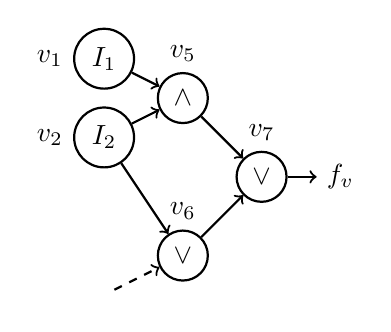
\begin{tikzpicture}[node distance={2cm and 2cm}, thick, scale=0.5, main/.style = {draw, circle}] 
			\node[main] (1) at (0,0) [label=west:$v_1$]{$I_1$}; 
			\node[main] (2) at (0,-2)[label=west:$v_2$] {$I_2$};
			\node (3) at (0,-4) {};
			\node (4) at (0,-6) {};
			
			\node[main] (5) at (2,-1)[label=north:$v_5$]{$\wedge$}; 
			\node[main] (6) at (2,-5)[label=north:$v_6$]{$\vee$};
			
			\node[main] (7) at (4,-3)[label=north:$v_7$]{$\vee$};
			
			\node (f) at (6,-3) {$f_v$};
			
			
			\draw[->] (1) -- (5);
			\draw[->] (2) -- (5);
			\draw[->] (2) -- (6);
			\draw[dashed, ->] (4) -- (6);
			\draw[->] (5) -- (7);
			\draw[->] (6) -- (7);
			\draw[->] (7) -- (f);
			
		\end{tikzpicture} 
	\label{subfig:OGD_sync_a}
	}
	\subfigure[OGD representation of the logic network]
	{
		\centering
		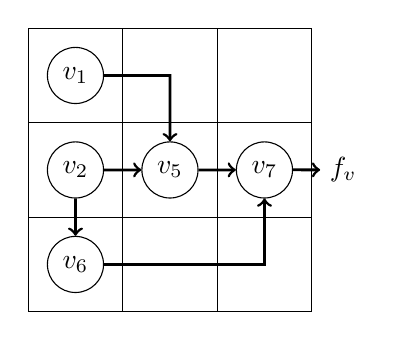
\begin{tikzpicture}[scale=1.2, main/.style = {draw, circle, fill=white}]
			
			\draw[fill=white]  (0, 2) -- (1, 2) -- (1,1) -- (0,1) -- cycle;
			\draw[fill=white]  (1, 2) -- (2, 2) -- (2,1) -- (1,1) -- cycle;
			\draw[fill=white]  (2, 2) -- (3, 2) -- (3,1) -- (2,1) -- cycle;
			
			
			\draw[fill=white]  (0, 3) -- (1, 3) -- (1,2) -- (0,2) -- cycle;
			\draw[fill=white]  (1, 3) -- (2, 3) -- (2,2) -- (1,2) -- cycle;
			\draw[fill=white]  (2, 3) -- (3, 3) -- (3,2) -- (2,2) -- cycle;
		
			
			\draw[fill=white]  (0, 4) -- (1, 4) -- (1,3) -- (0,3) -- cycle;
			\draw[fill=white]  (1, 4) -- (2, 4) -- (2,3) -- (1,3) -- cycle;
			\draw[fill=white]  (2, 4) -- (3, 4) -- (3,3) -- (2,3) -- cycle;
			
			
			\node[main] (1) at (0.5, 3.5) {$v_1$}; 
			\node[main] (2) at (0.5, 2.5) {$v_2$};

			\node[main] (5) at (1.5,2.5){$v_5$}; 
			\node[main] (6) at (0.5,1.5){$v_6$};
			
			\node[main] (7) at (2.5,2.5){$v_7$};
			
			\node [right of = 7] (f) {$f_v$};
			
			
			\draw[->, line width = 1pt] (1) -- (1.5, 3.5) -- (5);
			\draw[->, line width = 1pt] (2) -- (5);
			\draw[->, line width = 1pt] (2) -- (6);
			\draw[->, line width = 1pt] (5) -- (7);
			\draw[->, line width = 1pt] (6) -- (2.5, 1.5) -- (7);
			\draw[->, line width = 1pt] (7) -- (f);

			
			
		\end{tikzpicture}
		\label{subfig:OGD_sync_b}
	}
	\subfigure[No sufficient clocking for this OGD can be examined]
	{
		\centering
		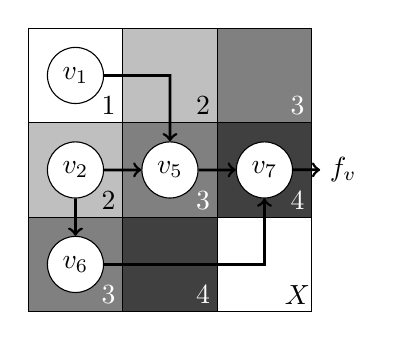
\begin{tikzpicture}[scale=1.2, main/.style = {draw, circle, fill=white}]
			
			\draw[fill=gray]  (0, 2) -- (1, 2) -- (1,1) -- (0,1) -- cycle;
			\draw[fill=darkgray]  (1, 2) -- (2, 2) -- (2,1) -- (1,1) -- cycle;
			\draw[fill=white]  (2, 2) -- (3, 2) -- (3,1) -- (2,1) -- cycle;
			
			
			\draw[fill=lightgray]  (0, 3) -- (1, 3) -- (1,2) -- (0,2) -- cycle;
			\draw[fill=gray]  (1, 3) -- (2, 3) -- (2,2) -- (1,2) -- cycle;
			\draw[fill=darkgray]  (2, 3) -- (3, 3) -- (3,2) -- (2,2) -- cycle;
			
			
			\draw[fill=white]  (0, 4) -- (1, 4) -- (1,3) -- (0,3) -- cycle;
			\draw[fill=lightgray]  (1, 4) -- (2, 4) -- (2,3) -- (1,3) -- cycle;
			\draw[fill=gray]  (2, 4) -- (3, 4) -- (3,3) -- (2,3) -- cycle;
			
			\node[text=white] (A1) at (0.85,1.18) {$3$};
			\node[text=white] (A1) at (1.85,1.18) {$4$};
			\node[text=black] (A1) at (2.85,1.18) {$X$};
			
			
			\node[text=black] (A1) at (0.85,2.18) {$2$};
			\node[text=white] (A1) at (1.85,2.18) {$3$};
			\node[text=white] (A1) at (2.85,2.18) {$4$};
			
			
			\node[text=black] (A1) at (0.85,3.18) {$1$};
			\node[text=black] (A1) at (1.85,3.18) {$2$};
			\node[text=white] (A1) at (2.85,3.18) {$3$};
			
			\node[main] (1) at (0.5, 3.5) {$v_1$}; 
			\node[main] (2) at (0.5, 2.5) {$v_2$};
			
			\node[main] (5) at (1.5,2.5){$v_5$}; 
			\node[main] (6) at (0.5,1.5){$v_6$};
			
			\node[main] (7) at (2.5,2.5){$v_7$};
			
			\node [right of = 7] (f) {$f_v$};
			
			
			\draw[->, line width = 1pt] (1) -- (1.5, 3.5) -- (5);
			\draw[->, line width = 1pt] (2) -- (5);
			\draw[->, line width = 1pt] (2) -- (6);
			\draw[->, line width = 1pt] (5) -- (7);
			\draw[->, line width = 1pt] (6) -- (2.5, 1.5) -- (7);
			\draw[->, line width = 1pt] (7) -- (f);
			
			
			
		\end{tikzpicture}
		\label{subfig:OGD_sync_c}
	}
	
	\caption{Insufficient timing constraints of a OGD representation \cite{Walter}}\label{fig:OGD_timing}
\end{figure}

The idea used for the ortho algorithm comes from an extension to OGDs, which allows to determine a special OGD from a logic network in polynomial time being the constraint needed for a scalable approach. The base used in \cite{ortho} is formed by Therese Biedl \cite{biedl1998better}, who proposes a OGD with an additional edge coloring. Although the effectiveness and complexity bounds in her work were proven on the restriction of \textit{undirected 3-graphs} and as we already examined from the precious chapter a logic network is neither containing only nodes of most degree 3 nor undirected. To overcome the fist restriction, a custom logic network can be created by assigning own nodes for fan-outs and inverters. This way the maximum node degree gets decreased to three, while the expressiveness of the logic network representation is maintained. The second restriction can be overcome by a custom coloring built on the original approach, which also serves as direction assignment. Given a logic network converted to a 3-graph, the coloring in form of edge directions $d : \Delta \rightarrow \{east, south\}$ is assigned. The coloring can be understood as relative position arrangement. If an edge $(v_i, v_j)$ is colored $east$, means that the vertex $v_j$ is positioned east of $v_i$, so that $x_j > x_i$. The color $south$ for an edge $(v_i, v_j)$ assigns $v_j$ a relative position of $v_i$, so that $v_j$ is south of $v_i$ or $y_j > y_i$. In order to color a graph with only these two colors the following \textit{assignment constraints} must hold true:

\begin{enumerate}
	\item All \textbf{incoming} edge of a vertex has to be painted with the \textbf{same} color.
	\item All \textbf{outgoing} edges of a vertex have to be painted with \textbf{opposite} colors.
\end{enumerate}

\begin{figure}
	\centering
	\subfigure[Color assignment of incoming signals]
	{
		\centering
		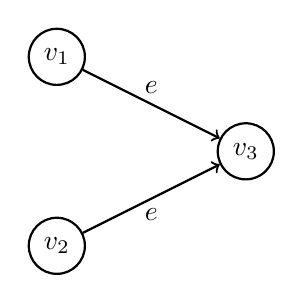
\begin{tikzpicture}[node distance={2cm and 2cm}, thick, scale=1.2, main/.style = {draw, circle}] 
			\node[main] (1) at (0,0) {$v_1$}; 
			\node[main] (2) at (0,-2){$v_2$};
			
			\node[main] (3) at (2,-1){$v_3$}; 
			
			\draw[->, above] (1) -- (3) node [midway] {$e$};
			\draw[->, below] (2) -- (3) node [midway] {$e$};
			
		\end{tikzpicture} 
		\label{subfig:OGD_color_out}
	}
	\subfigure[Color assignment of outgoing signals]
	{
		\centering
		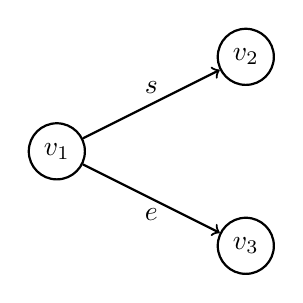
\begin{tikzpicture}[node distance={2cm and 2cm}, thick, scale=1.2, main/.style = {draw, circle}] 
			\node[main] (1) at (0,-1) {$v_1$}; 
			\node[main] (2) at (2,0){$v_2$};
			
			\node[main] (3) at (2,-2){$v_3$}; 
			
			\draw[->, above] (1) -- (2) node [midway] {$s$};
			\draw[->, below] (1) -- (3) node [midway] {$e$};
			
		\end{tikzpicture} 
		\label{subfig:OGD_color_in}
	}
	
	\caption{Relative positions of an OGD graph with correct color assinment}\label{fig:OGD_color}
\end{figure}

The relative position assignment under the proposed constraints can be seen at an arbitrary example in figure \ref{fig:OGD_color}. In the example for outgoing edges (figure \ref{subfig:OGD_color_out}), the assignment constraint makes sure that two outgoing edges of the same vertex are routed in different directions to avoid a conflict. Equivalent to the definition of the colors, the layout is increased in x-direction for an east-coloring and analogously extended in the y-Direction for a south-coloring. Figure \ref{subfig:OGD_color_in} depicts the assignment constraint for the incoming edges of one vertex. This assignment has to use one color and the node can be set non-conflicting for both incoming nodes in the layout by extending it in x-direction based on the east-coloring. However, there exist logic networks for which no coloring in regards to the constraints can be found. When such a coloring conflict appears, the conflicting edge, for which no direction can be assigned after the formulated constraints is divided and an auxiliary node is introduced resolving the conflict.
In order to allow data to propagate, ortho needs to map a valid clocking onto the layout. 
Because ortho uses OGDs with exactly two directions $east$ and $south$, the 2DDWave scheme, which also supports the data flow in exactly two directions, is perfectly suited for the algorithm. Also the usage of a predefined clocking scheme already gives a solution for the local synchronization constraint and due to the uniformity and simplicity of the 2DDWave scheme also the global synchronization constraint for nodes placed and routed after the proposed direction assignment is maintained.

\begin{figure}
	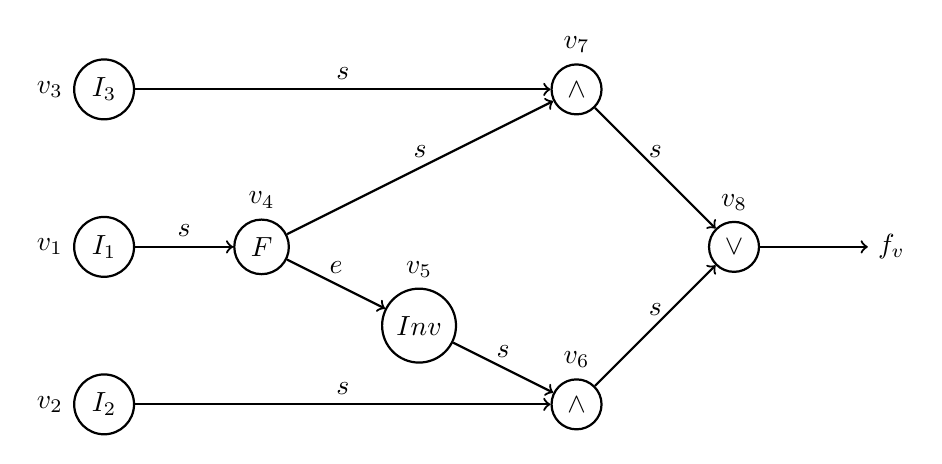
\begin{tikzpicture}[node distance={2cm and 2cm}, thick, scale=1, main/.style = {draw, circle}] 
		\node[main] (3) at (0,0) [label=west:$v_3$]{$I_3$}; 
		\node[main] (1) at (0,-2)[label=west:$v_1$] {$I_1$};
		\node[main] (2) at (0,-4)[label=west:$v_2$] {$I_2$};
		
		\node[main] (4) at (2,-2)[label=north:$v_4$]{$F$}; 
		
		\node[main] (5) at (4,-3)[label=north:$v_5$]{$Inv$};
		\node[main] (6) at (6,-4)[label=north:$v_6$]{$\wedge$};
		\node[main] (7) at (6,0)[label=north:$v_7$]{$\wedge$};
		
		\node[main] (8) at (8,-2)[label=north:$v_8$]{$\vee$};
		
		\node (f) at (10,-2) {$f_v$};
		
		
		\draw[->, above] (1) -- (4) node [midway] {$s$};
		\draw[->, above] (2) -- (6) node [midway] {$s$};
		\draw[->, above] (3) -- (7) node [midway] {$s$};
		\draw[->, above] (5) -- (6) node [midway] {$s$};
		\draw[->, above] (4) -- (5) node [midway] {$e$};
		\draw[->, above] (4) -- (7) node [midway] {$s$};
		\draw[->, above] (6) -- (8) node [midway] {$s$};
		\draw[->, above] (7) -- (8) node [midway] {$s$};
		\draw[->, above] (8) -- (f) node [midway] {};
		
		
	\end{tikzpicture}
	\caption{Logic Network of a 2:1 MUX after fan-out substitution,	inverter insertion and coloring}\label{fig:mux_LN}
\end{figure}

In the following the pseudo code of ortho, derived from \cite{ortho} is depicted as algorithm~\ref{alg:ortho} and described in own words, before its evaluated on an example and its main characteristics are described. Following the VLSI design process the ortho algorithm has as input a Logic network $N$ and a clocking scheme or rather a clock number $clk$ for every tile in order to fulfill the timing constraints. As already mentioned $N$ has to be converted into a 3-graph by substitution so a valid coloring can be assigned. The corresponding logic network for a 2:1 MUX can be seen in figure~\ref{fig:mux_LN}. Then an empty Layout $L$ with a 2DD-Wave clocking scheme is created and the coloring is calculated for $N$. Also the nodes need to be topologically ordered starting with the lowest number at the inputs and the highest numbers at the outputs. Therefore, the algorithm is starting with the lowest numbered vertices representing primary inputs. In order to connect the inputs to external signals they are placed at the borders of the layout. In ortho, the first column of the layout is therefore reserved for placing the inputs under each other. Due to the properties of OGD, a conflict arises, when inputs have outgoing edges colored south, because the algorithm would then wire these edges into y-direction and therefore over other primary inputs. Since this is forbidden in OGD and for QCA layouts, these conflicts need to be resolved by the algorithm. To do so, primary inputs colored $south$ are resolved by first rewiring them each on a new column, allowing a wiring into y-Direction and thus the placement of the nodes connected to their outgoing edges. Further, for the placement and routing of all nodes in the logic network, the two parameters coloring and the updated parameter $(w, h)$, saving the current dimensions of $L$, need to be evaluated in each step. So if a node is colored $east$, the layout is extended by one column and the node is placed at $(w-1, h_p)$, where $w$ is the current width of $L$ and $h_p$ is the maximum vertical position of its childs. According to this scheme for nodes colored $south$ the layout is extended by one row and the node is placed to $(w_p, h-1,)$, where $w_p$ is the maximum horizontal position of the nodes childs and $h$ is the current height of the layout. After placing the node, it is wired to its predecessors, while the placement into a new row or column makes sure the wiring doesn't pass over another gate. If only one predecessor exists the wiring also goes only $south$ or $east$. But when two predecessors exist, in case of $east$ the predecessor giving $h_p$ is also only wired in x-Direction, while the other predecessor has to be wired with two wire segments, the first also going into x-Direction and the second one connecting in y-Direction. If the node is colored $south$ the two segment wiring goes south first and then east. After all nodes were placed in this fashion the primary outputs are also connected to the borders either to the east or the south and the finished layout $L$ is returned by the algorithm.



%\begin{figure}
%	\centering
%	\includegraphics[scale=0.7]{Coloring_conflict}
%	\caption{Solution for a coloring conflict}\label{fig:Coloring_conflict}
%\end{figure}

\algnewcommand\algorithmicforeach{\textbf{for each}}
\algdef{S}[FOR]{ForEach}[1]{\algorithmicforeach\ #1\ \algorithmicdo}
\begin{algorithm}[H]
	\hspace*{\algorithmicindent} \textbf{Input:} Logic network $N$ \\
	\hspace*{\algorithmicindent} \textbf{Input:} Clock number $clk$\\
	\hspace*{\algorithmicindent} \textbf{Output:} Gate level layout $L$
	\begin{algorithmic}[1]
		\State Convert $N$ to a 3-graph by substitution
		\State $L \leftarrow$ empty 2DDWave-clocked layout of size $w = 0 \times (h = 0)$
		\State Generate direction assignment $d : \Delta \rightarrow \{east, south\}$ and subdivide signals if necessary
		\State Compute topological ordering $v_1, . . . , v_i \in N$
		\State Extend $L$ by one column and reserve it for primary inputs
		\ForAll {vertex $v_1, ..., v_i \in N $ with at most two incoming signals $\sigma_1, \sigma_2$}
		\If{vertex $v$ is terminal/primary input}
		{
			\State Extend $L$ by one row
			\State Place v at position $(0, h - 1)$
			\If{vertex $v$ is colored $south$}
				\State Extend $L$ by one column
				\State Wire the primary input to position $(w - 1, h - 1)$ 
			\EndIf
		}
		\ElsIf{$d(\sigma_1) = d(\sigma_2) = east$}
			\State Extend $L$ by one column
			\State $h_p \leftarrow$ max. vertical position of v's predecessors
			\State Place v at position $(w - 1, h_p)$
		\ElsIf { signals are labeled $south$}
			\State Extend $L$ by one row
			\State $w_p \leftarrow$ max. horizontal position of v's predecessors
			\State Place v at position $(w _p, h - 1)$
		\EndIf
			\State Draw orthogonal wire segments to connect v with its predecessor(s) accordingly 
		\EndFor
		\State Connect the primary outputs to the respective borders\\
		\Return $L$
	\end{algorithmic}
	\caption{Ortho algorithm}\label{alg:ortho}
\end{algorithm}

The example depicted in figure \ref{fig:ortho_mux_21} shows the $(p, r, c)$ of a 2:1 MUX. As a reminder, the logic network is depicted in figure~\ref{fig:mux_LN}. Starting with a layout of size $(1, 0)$, for the PI $v_1$, the layout is extended by one column to $(1, 1)$ and is placed to $(0, h-1) = (0, 0)$. Because the outgoing edge of the PI is labeled $south$, the wiring has to be resolved by extending $L$ to $(2, 1)$ and wiring the PI to $(w-1, h-1)=(1, 0)$. For the other PIs $v_2, v_3$ it follows the placement to $(0, 1)$ and $(0, 2)$ and an increase of one column per PI since they have both outgoing edges labeled south. The resolving wiring leads to $(2, 1)$ and $(3, 2)$. Now the remaining nodes can be placed following the $east, south$ scheme. The size of the layout after the input network is $(4, 3)$. With $v_4$ a fan-out node is placed south of the third input, which has coordinates $(3, 2)$. After extending $L$ by one row, the y-coordinate is evaluated to be $w-1 = 3$ and the x-coordinate $3$ is adopted from its only predecessor. Therefore, the node is placed on $(3, 3)$ and $L=(4, 4)$. In the same fashion the parent node of the fan-out $v_5$, representing an inverter is placed east of it. So the coordinates of the inverter are $(4, 3)$ and $L = (5, 4)$. Looking at the next node $v_6$, which is the first node with two children and which is labeled south now the x-coordinate is determined by the eastern predecessor, so $v_5 = (4, 3)$. The y-coordinate is again adapted form the size of the layout, after it was increased in y-direction once, resulting in a placement on $(4, 4)$ and $L = (5. 5)$, The same way the AND-node $v_7 = (3, 5)$ ($L = (5, 6)$) and the OR-node $v_8 = (4, 6)$ ($L = (5, 7)$) are placed. Since all nodes are placed now the primary output has to be placed from $v_8$. For this the layout is increased by one column again ($L = (6, 7)$) and the PO is placed to the eastern border.

\begin{figure}
	\centering
	\includegraphics[scale=0.5]{ortho_mux_21}
	\caption{Placement and routing of a 2:1 mux network using the ortho algorithm}\label{fig:ortho_mux_21}
\end{figure}

From the returned layout we can see that the signal flow is straight forward in south-eastern direction due to the 2DD-Wave clocking scheme the algorithm is bound to and as already discussed in the section about clocking \ref{subsec:clocking}, this limits ortho in many ways. First of all due to the selection of the "+"-majority gate as standard gate, they cannot be placed on the 2DD-Wave scheme, because the clocking only allows two-input logic gates. Also back-loops are not allowed in the clocking, prohibiting the placement and routing of sequential circuits. Though, ortho provides an efficient tool for the placement and routing of purely combinational circuits. As shown in paper \cite{walter2018exact}, the 2DD-Wave scheme provides the most area efficient clocking when it comes to combinational circuits, beating both the USE and RES scheme.

With a deep understanding of the ortho algorithm with its constraints, involving drawbacks and advantages, now other ideas with comparable approaches or based on the ortho algorithm can be discussed. \textit{Ropper}, a placement and routing framework \cite{ropper} proposes an algorithm, which is based on \cite{trindade2016placement}. As already discussed in the part about preprocessing, this algorithm brings some disadvantages, because dummy nodes are inserted as part of logic synthesis, leading to an increased size of the logic network. In ortho this step is unnecessary. Nevertheless the authors of Ropper point out that they have overcome some restrictions of ortho, one of them being able to place majority gates and also a more area efficient placement and routing. But these improvements come at a price. First of all the framework only achieves the placement and routing of majority gates not because of a clocking scheme providing three input tiles to a given tile, but supporting the use of rotated majority gates, which had been discussed to be very prone to crosstalk. Also custom gates and double wiring is used, so that many tiles have QCA cells placed only with a distance of one cell and not like \cite{crosstalk} suggests a minimum distance of two QCA cells. The use of these custom gates is necessary in this algorithm, because the design used doesn't rely on the same strict constraints as ortho. The Ropper framework even routes wires above gates (solved with custom tiles) and doesn't use border inputs and outputs making it challenging to input and read data from the circuit. Based on the argumentation used in this work, the Ropper framework violates to many design rules, which have been analyzed to be necessary for a sufficient placement and routing algorithm.

Another paper trying to implement majority gates for QCA is \textit{migortho}, which is based on the ortho algorithm provided in fiction. The difference of the algorithms is the use of the underlying gate-library. While this work uses the same as ortho, migortho utilizes the QCA-ONE library. From the preliminaries, it is already known that again the use of rotated majority gates and therefore the use of double wires is allowed. This means that circuits designed by migortho are also being considered to be prone to crosstalk, following the argumentation from above. But the algorithm shows that with the use of a different library ortho is already powerful enough to overcome some restrictions. This fact has motivated this work to implement some different ideas to enable ortho to be more area efficient, place "+"-majority gates and even implement a strategy for the automated placement and routing of sequential circuits.

\section{Design of Sequential QCA circuits}
In this section the state of the art for sequential circuit design in QCA is discussed. Compared to the algorithms existent for the placement and routing for combinational logic, this area is still in its infancy. This section first focuses on the main part of implementing sequential logic and then uses this knowledge to give an insight into the implementation of storage cells. 

\subsection{Sequential logic in QCA}
In recent literature, several attempts have been made to implement latches and flip-flops (FFs) in order to obtain storage elements and enable sequentiality for quantum-dot cellular automata (QCA) circuits \cite{sequential_cell_one, sequential_cell_two, dual_edge_triggered_FF_cell, sequential_reversible_cell}. These works primarily aim to translate Boolean CMOS equations into majority representations and implement this representation using QCA gates. However, the resulting circuits often rely on external 2-phase clocking signals adopted from the CMOS domain \cite{sequential_cell_one}, despite the fact that QCA circuits already employ 4-phase clocking. The authors of \cite{sequential_cell_two} argue that a latching can be accomplished using QCA clocking, but that this would lead to a restriction of the circuit. However, as discussed in the subsections on clocking (\ref{subsec:clocking}) and storage elements (\ref{subsec:latchesandregisters}), it is suggested that the external clocking signal may be unnecessary and that the 4-phase clocking of QCA circuits should be used to accomplish sequential functionalities.

While some works propose more advanced sequential circuits, such as dual edge-triggered D-FFs \cite{dual_edge_triggered_FF_cell} and reversible latches \cite{sequential_reversible_cell}, they still rely on cell-based clocking, which was found to be insufficient in subsection \ref{subsec:clocking}. The USE clocking scheme \cite{USE} has been proposed as an evolution towards sequential tile-based placement and routing, but leads to worse layouts compared to 2DD-Wave for most benchmark problems \cite{walter2018exact}. Other works, such as \cite{sequential_reversible_tile} and \cite{sequential_tile_CMOS_alg}, propose different latches and sequential element implementation algorithms using the USE scheme. However, these approaches all share the drawback of translating sequential logic directly from the CMOS domain.

As previously discussed in this work, wire segments should be used as storage elements as proposed in \cite{Walter}. However, this work does not provide any circuits or placement and routing algorithms using these elements. In this work, the basic ideas of wire delays are utilized and adjusted according to the placement and routing of QCA circuits.

\subsection{QCA storage cells (QCA RAM)}\label{subsec:RAM_SoA}
Another area of research in QCA technology focuses on the implementation of random access memory (RAM) cells. While this paper primarily focuses on a placement and routing algorithm for sequential logic, the implementation of QCA storage can also be adapted. The current state of the art can be divided into two approaches for implementing RAM in QCA.

The first approach, as presented in the papers \cite{RAM_overview, crosstalk, RAM_cell}, involves translating CMOS technology into QCA and thus dealing with the same shortcomings resulting from an external clock signal. Additionally, these circuits are also based on cell-based clocking, which is insufficient for this work.

The second approach, as presented in \cite{ahmad2018optimal, majeed2019optimal}, proposes the use of multiplexer (MUX) structures to implement RAM cells. By using a 2:1 MUX with a RAM cell holding one bit of information and a bitline (BL) also holding one bit as inputs, the 2:1 MUX can decide whether the information on the BL is passed into the RAM cell or if the information in the RAM cell is retained, based on the information on the wordline (WL) which serves as the third input to the 2:1 MUX. However, the implementations shown in \cite{ahmad2018optimal} and \cite{majeed2019optimal} still use an external clock signal and are also clocked cell-based.

The ideas of wire delays can be combined with the use of MUX to build a RAM cell, which can be constructed using orthogonal and the corresponding sequential distribution network, as proposed later in this work.
